
\فصل{کارهای پیشین}

 کار‌های پیشین انجام‌شده در حوزه‌ی ASPECTS از چند نظر قابل بررسی و مقایسه هستند.
اولین دیدگاه، روش مورد استفاده در این کارها است.
دیدگاه دیگر نیز مجموعه‌داده و منابع مورد دسترسی این پژوهش‌ها می‌باشد.
بررسی کار‌های پیشین از این دو دیدگاه، این مزیت را دارد 
که جایگاه پروژه حاضر را بیشتر مشخص می‌کند و محدودیت‌ها و کارآمدی‌های آن را 
بهتر شرح می‌دهد.
در این فصل، پژوهش‌های پیشین در این چهارچوب، مورد تحلیل قرار می‌گیرند.

\قسمت{روش‌های مورد استفاده}
کارهای پیشین انجام شده از نظر روش مورد استفاده، در چند دسته‌ی کلی قابل بررسی هستند.
در طی بررسی هر دسته، ابتدا روش کلی مورد استفاده در آن توضیح داده می‌شود. 
سپس به نمونه‌هایی از کارهای پیشین که در آن چهارچوب کار کرده‌اند اشاره می‌شود
و نتایج به‌دست آمده توسط این کار‌ها عنوان شده و مورد مقایسه قرار می‌گیرد.

\زیرقسمت{روش ناحیه‌بندی و طبقه‌بندی}
در این روش، ده بخش مورد توجه ASPECTS در تصاویر مغزی، 
ناحیه‌بندی\footnote{Segmentation}
 می‌شوند.
به این ترتیب،  
مدل یادگیری ماشین به طور مستقیم از محل این نواحی در تصاویر آگاهی می‌یابد.
سپس مدل آموزش داده‌می‌شود که هر ناحیه‌ای که می‌بیند، آیا آسیب دیده‌است یا خیر.
یعنی یاد می‌گیرد که هر ناحیه را به دو دسته‌ی آسیب‌دیده و سالم 
طبقه‌بندی\footnote{Classification}
کند.
سپس با جمع امتیازات تمام ده ناحیه‌ی هر بیمار، امتیاز ASPECTS وی به‌دست می‌آید.

\زیرزیرقسمت{ناحیه‌بندی نواحی ASPECTS}

ناحیه‌بندی ۱۰ بخش ASPECTS تصاویر به دو طریق مختلف انجام می‌شود.
روش اول از یادگیری ماشین بهره می‌گیرد.
در این روش، هر تصویر مغزی، برچسبی دارد که نشان می‌دهد کدام پیکسل‌های تصویر متعلق به هر ناحیه هستند.
تعداد زیادی از تصاویر مغزی به همراه این برچسب‌ها به مدل ورودی داده تا ناحیه‌بندی را بیاموزد.
به این ترتیب، مدل می‌تواند با دریافت یک تصویر مغزی جدید و بدون برچسب، مشخص کند که کدام پیکسل‌ها متعلق به هر ناحیه هستند.

روش دیگر ناحیه‌بندی، مبتنی بر یادگیری نیست و نیازی به تعداد زیادی تصویر به همراه برچسب ندارد.
بلکه در این روش، یک یا چند تصویر مغزی استاندارد، به عنوان 
الگو\footnote{Template}
برچسب زده می‌شوند.
سپس به کمک روش‌های 
انطباق تصاویر،\footnote{\lr{Image Registration}}
تصویر الگو بر یک تصویر مغزی مورد نظر منطبق می‌شود تا نواحی مشخص شده روی آن، در تصویر جدید هم مشخص شوند.

از جمله روش‌های منطبق کردن تصویر الگو بر روی تصویر جدید، جابجایی، دوران، بزرگ‌نمایی، تغییر شکل جزئی و \dots می‌باشد.
تصویر الگو آن‌قدر دچار این دست تغییرات می‌شود تا معیار شباهتش با تصویر جدید به حد مطلوبی برسد.
یک نمونه‌ی ساده از چنین معیاری می‌تواند مجموع اختلاف قدر مطلق دو تصویر باشد که باید کمینه شود.
لازم به ذکر است که روش‌های ناحیه‌بندی به کمک انطباق تصاویر، عموماً توانایی کمتری نسبت به مدل‌های 
یادگیری ماشین دارند اما نسبت به آن روش‌ها نیازمندی‌های داده‌ای کمتری دارند.

\زیرزیرقسمت{استخراج ویژگی نواحی}
پس از مشخص شدن محدوده‌ی هر ناحیه‌ی ،ASPECTS لازم است ویژگی‌های اصلی هر ناحیه استخراج شود تا مدل بتواند از روی این ویژگی‌ها، آن ناحیه را دسته‌بندی کند.
در کارهای پیشین، محاسبه‌ی چنین ویژگی‌هایی به دو طریق مختلف انجام شده‌است.
دسته‌ی اول، استخراج ویژگی‌های هر ناحیه را به مدل یادگیری ماشین واگذار می‌کنند.
یعنی تصاویر به مدل، ورودی داده می‌شوند و مدل طی چندین مرحله مشاهده‌ی نواحی به همراه برچسبشان، می‌آموزد که چه ویژگی‌هایی از تصاویر استخراج کند که بیش از همه مفید باشند.

اما دسته‌ی دیگر برای استخراج ویژگی تصاویر، به جای یادگیری ماشین، روش‌های محاسباتی و پردازش تصویری را به‌کار می‌گیرند.
در واقع یک‌سری ویژگی‌های آماری همچون میانگین و واریانس شدت رنگ پیکسل‌ها برای هر ناحیه محاسبه می‌شوند.
پس از اینکه این ویژگی‌ها برای هر ناحیه استخراج شدند، 
در اختیار مدل یادگیری ماشین یا هوش مصنوعی قرار می‌گیرند
تا 
در طبقه‌بندی نواحی، استفاده شوند.

\زیرزیرقسمت{نمونه‌ی کارهای پیشین}
یکی از تازه‌ترین پژوهش‌ها در زمینه‌ی امتیاز‌دهی خودکار ،ASPECTS در همین دسته‌ از روش‌ها قرار می‌گیرد \cite{lee2023clinical}.
این پژوهش با ناحیه‌بندی نواحی ASPECTS و استخراج ویژگی‌های نواحی به کمک مدل یادگیری ماشین، توانسته به دقت های نسبتاً خوبی 
(تشخیص\footnote{Specificity}
۶۳٪.۹۶
و
حساسیت\footnote{Sensitivity}
۷۸٪.۶۲
در امتیازدهی ده‌گانه و 
تشخیص
۵۶٪.۷۶
و
حساسیت
۴۲٪.۹۵
در امتیازدهی دوبخشی 
)
دست یابد.
نمونه‌ی موفق و اخیر دیگری وجود دارد که نواحی را به کمک یادگیری ماشین ناحیه‌بندی و طبقه‌بندی می‌کند \cite{cao2022deep}.
این نمونه نیز نتایج بسیار خوبی 
(تشخیص
۲٪.۹۲
و
حساسیت
۲٪.۷۷
در امتیازدهی ده‌گانه و 
تشخیص
۶٪.۸۶
و
حساسیت
۵٪.۹۵
در امتیازدهی دوبخشی 
)
گزارش کرده‌است.
کار دیگری
\cite{kuang2021eis}
که ناحیه‌بندی را به کمک انطباق تصاویر انجام داده است،
برای امتیازدهی ده‌گانه و دو‌بخشی به ترتیب دقت
۸۴٪ 
و 
۹۰٪ 
را گزارش کرده‌است.
همچنین یک نمونه از قدیمی‌ترین کار‌های پیشین که دو روش برای محاسبه‌ی ASPECTS پیشنهاد داده، در روش ناحیه‌بندی و طبقه‌بندی خود،  
دقت
۹٪.۷۰
را اعلام کرده است \cite{jung2018evaluating}.

چند نمونه کار پیشین نیز در ادامه عنوان می‌شود که در استخراج ویژگی‌های نواحی، از روش‌های آماری استفاده کرده‌اند.
یکی از موفق‌ترین نمونه‌ها در این دسته، پژوهشی نسبتاً قدیمی است که
تشخیص
۸٪.۹۱،
حساسیت
۲٪.۶۶
و دقت 
۹٪.۸۴
در امتیازدهی ده‌گانه و 
تشخیص
۸۰٪،
حساسیت
۸٪.۹۷
و دقت 
۹۶٪
را
در امتیازدهی دوبخشی 
به‌دست آورده‌است \cite{kuang2019automated}.
نمونه‌های دیگری نیز از سال‌های اخیر وجود دارند
\cite{liu2021deep,yu2021automated}
که به علت مقایسه‌پذیر نبودن و یا ابهام در روش اعتبارسنجی، از ذکر نتایج آن‌ها صرف نظر می‌شود.

\زیرقسمت{روش ناحیه‌بندی و هم‌پوشانی}
در این روش، دو نوع ناحیه‌بندی انجام می‌شود.
نوع اول، نواحی ASPECTS و نوع دوم،
بخش‌های آسیب‌دیده‌ی مغزی در اثر انسداد عروق 
را مشخص می‌کند.
سپس هم‌پوشانی بخش‌های آسیب‌دیده با هر ناحیه محاسبه می‌شود.
در صورتی که نسبت مساحت آسیب‌دیده‌ی یک ناحیه، از یک حد آستانه فراتر برود، آن ناحیه به عنوان آسیب‌دیده گزارش می‌شود و در غیر این صورت، سالم شناخته می‌شود.
در واقع در این روش‌ها، مدل‌های یادگیری ماشین، وظیفه‌ی اصلی ناحیه‌بندی را بر عهده دارند و نه طبقه‌بندی.

واضح است که ناحیه‌بندی نواحی آسیب‌دیده، بر خلاف ناحیه‌بندی نواحی ده‌گانه‌ی ،ASPECTS
به روش انطباق تصاویر ممکن نیست.
زیرا الگوی ثابت و مشخصی برای نواحی آسیب‌دیده وجود ندارد.
به همین دلیل این روش‌ها برای آموزش مدل ماشین، عموماً نیازمند تعداد زیادی تصویر مغزی به همراه برچسب پیکسل‌های آسیب‌دیده هستند.
این نوع از برچسب‌ها، وقت و انرژی زیادی از نیرو‌های انسانی می‌گیرند و تهیه‌ی آن‌ها دشوارتر است.

\زیرزیرقسمت{نمونه‌ی کارهای پیشین}

در میان کارهای پیشین،
سه پژوهش با
روش ناحیه‌بندی و هم‌پوشانی
یافته‌شد.
یکی از بهترین نتایج 
گزارش‌داده‌شده مربوط به پژوهشی در سال ۲۰۲۱ است
\cite{naganuma2021alberta}
که
تشخیص
۹۷٪،
حساسیت
۸۰٪
و دقت 
۹۶٪
در امتیازدهی ده‌گانه و 
تشخیص
۹۲٪،
حساسیت
۹۸٪
و دقت 
۹۷٪
را
در امتیازدهی دوبخشی 
گزارش کرده‌است.
البته در این پژوهش به وضوح اشاره نشده‌است که این نتایج مربوط به داده‌های آموزشی هستند و یا آزمایشی.
در پژوهش دیگری
تشخیص
۱۷٪
تا
۸۳٪
و
حساسیت
۶۹٪
تا
۱۰۰٪
در امتیازدهی نواحی ده‌گانه و 
تشخیص
۴۸٪
تا
۹۳٪
و
حساسیت
۷۴٪
تا
۹۹٪
در یک امتیازدهی سه‌بخشی 
ارائه شده‌است \cite{naganuma2021alberta}.
آخرین مورد مطالعه‌شده نیز نتایج را در قالب 
بهبودی که در توانایی تشخیصی متخصصان ایجاد می‌کند ذکر کرده‌است و از آن عبور می‌شود \cite{chen2022improving}.

\زیرقسمت{روش کل‌نگری و طبقه‌بندی}
تعداد بسیار محدودی از پژوهش‌ها در این دسته قرار می‌گیرند
که پژوهش حاضر نیز یکی از آن‌ها است.
در این روش، تنها با در دست داشتن امتیاز ASPECTS کلی بیمار، امتیاز ASPECTS تصاویر فراگرفته می‌شود.
در واقع در این روش، مدل تعداد زیادی تصویر مغزی به همراه برچسب امتیاز نهایی ASPECTS آن‌ها را مشاهده می‌کند و 
نمونه‌های جدید تصاویر مغزی را در یکی از دسته‌های امتیاز
ASPECTS
طبقه‌بندی می‌کند.

در فصل بعد خواهد آمد که این دسته از روش‌ها کمترین نیاز‌مندی داده‌ای را دارند.
به همین نسبت، دقت این روش‌ها نسبت به روش‌های قبلی، عموماً پایین‌تر است.
با این حال، پژوهشی
\cite{golkonda2022automated}
وجود دارد که در این دسته از روش‌ها، بالاترین دقت 
در میان تمام کارهای پیشین
را گزارش کرده‌است.
طبق بررسی‌های انجام شده، نتایج گزارش‌شده معتبر نیستند
چرا که در ارزیابی مدل، جدایی میان داده‌های آموزشی و آزمایشی رعایت نشده‌است.
به عبارتی ارزیابی شامل داده‌هایی می‌شود که مدل، قبلا پاسخ آن‌ها را مشاهده کرده‌است و طبعاً پیش‌بینی درست‌تری روی آن خواهد داشت.
لذا از ذکر و مقایسه‌ی نتایج این پژوهش صرف نظر می‌شود.

به این ترتیب تنها یک نمونه کار دیگر با این روش در ادبیات موضوع باقی می‌ماند \cite{jung2018evaluating}.
این مدل، امتیاز ASPECTS را برای دو برش اصلی مغز می‌آموزد.
این پژوهش، خطای متوسط ۱۱۱۶.۰ و خطای واریانس 5080.2 را گزارش کرده‌است.

\زیرقسمت{سایر روش‌ها}
طبیعتاً روش‌های محاسبه‌ی خودکار ASPECTS محدود به روش‌های پیشنهادی فوق نیست
و هر پژوهشی را نمی‌توان لزوما در یکی از این دسته‌ها قرار داد.
در میان کارهای پیشین نیز چنین موردی وجود دارد \cite{chen2022improving}.
این پژوهش که جزء کار‌های تازه‌تر است، روش جالبی را به کار برده‌است که ذکر آن خالی از لطف نیست.

در این پژوهش، نواحی ASPECTS ناحیه‌بندی می‌شوند.
سپس از دو ترفند 
پیش‌آموزش‌دادن\footnote{Pre-training}
و 
تنظیم دقیق\footnote{Fine Tuning}
برای آموزش مدل در دو مرحله استفاده می‌شود.
در گام اول، مدل با دریافت تعداد زیادی برش از مغز به همراه برچسب ASPECTS همان برش، پیش‌آموزش می‌بیند.
سپس این مدل، با دریافت تعداد زیادی تصویر با برچسب‌هایی در سطح هر ناحیه، تنظیم دقیق می‌شود.

این پژوهش نهایتاً تشخیص
۶٪.۸۱،
حساسیت
۲٪.۶۵
و دقت 
۷٪.۷۹
در امتیازدهی ده‌گانه و 
تشخیص
۷٪.۹۰،
حساسیت
۲٪.۷۲
و دقت 
۹٪.۸۸
را
در امتیازدهی دوبخشی 
گزارش می‌کند که می‌تواند در برخی کاربرد‌ها مناسب باشد.

\قسمت{مجموعه‌داده و برچسب مورد استفاده}
یک رویکرد دیگر برای مطالعه‌ی کارهای پیشین، بررسی آن‌ها از نظر مجموعه‌داده‌ی در دسترس و برچسب‌ها آن است.
در این قسمت، کارهای پیشین از این منظر با پژوهش حاضر مقایسه می‌شوند
و
محدودیت‌های داده‌ای این پروژه از این دیدگاه مورد تحلیل قرار می‌گیرد.

\زیرقسمت{حجم مجموعه‌داده}
در این پژوهش، پس از مرتب‌سازی، خالص‌سازی و حذف داده‌های نامناسب (مانند تصاویر با نویز بسیار زیاد)، مجموعا تصاویر ۱۰۰ بیمار آماده‌ی عرضه به مدل بودند.
هر یک از این بیماران، با توجه به وضعیت خود، یک امتیاز ASPECTS داشتند.
شکل \ref{fig:patient-count}، توزیع امتیاز ASPECTS این بیماران را نشان می‌دهد.
این تصویر نشان می‌دهد که در امتیازدهی دوبخشی ASPECTS در دسته‌ی امتیاز زیر ۶، در مجموع تنها ۱۱ بیمار وجود داشتند.
این در حالی است که امتیاز ۱۰، به تنهایی شامل ۳۱ بیمار می‌شد.
این موضوع علاوه بر حجم کوچک مجموعه‌داده، نشان از 
نامتوازن\footnote{Imbalanced} 
بودن آن دارد.

% \begin{figure}[ht]
% \centering
% 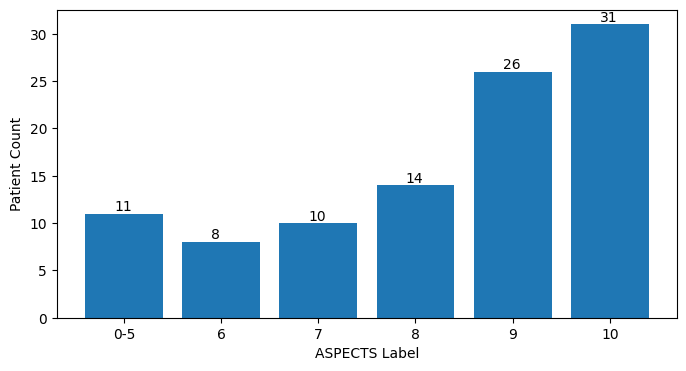
\includegraphics[width=\textwidth, keepASPECTSratio]{patient-count.png}
% \caption[]{توزیع امتیاز ASPECTS بیماران}
% \label{fig:patient-count}
% \end{figure}

\شروع{شکل}[ht]
\centerimg{patient-count}{\textwidth}
\شرح[توزیع امتیاز ASPECTS بیماران]{توزیع امتیاز ASPECTS بیماران}
\برچسب{fig:patient-count}
\پایان{شکل}

در مجموعه‌داده‌ی مورد استفاده در این پژوهش، برخی بیماران، چند نوبت تصویربرداری داشتند.
بنابراین به ازای برخی بیماران، بیش از یک تصویر وجود داشت.
تصاویر مختلف متعلق به یک بیمار، عموماً تفاوت‌های ظاهری اندکی داشتند اما شکل و شمایل ناحیه‌ی آسیب‌دیده در آن‌ها مشابه بود.
به این ترتیب، در مجموع، ۱۵۹ تصویر از ۱۰۰ بیمار در مجموعه‌داده حاضر بودند.
شکل \ref{fig:image-count} 
تعداد تصاویر موجود 
به ازای برچسب ASPECTS را نشان می‌دهد.

% \begin{figure}[ht]
% \centering
% 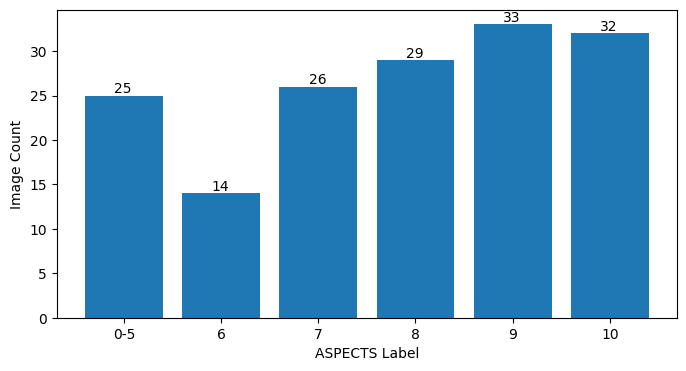
\includegraphics[width=\textwidth, keepaspectratio]{image-count.png}
% \caption[]{تعداد تصویر (نه کاملاً نو) به ازای هر امتیاز ASPECTS}
% \label{fig:image-count}
% \end{figure}

\شروع{شکل}[ht]
\centerimg{image-count}{\textwidth}
\شرح[تعداد تصاویر به ازای امتیاز ASPECTS]{تعداد تصویر (نه کاملاً نو) به ازای هر امتیاز ASPECTS}
\برچسب{fig:image-count}
\پایان{شکل}

این تعداد تصویر به خصوص در برخی امتیاز‌های ،ASPECTS تعداد کمی محسوب می‌شود.
این موضوع از مقایسه‌ی حجم مجموعه‌داده‌ی در اختیار این پژوهش با مجموعه‌داده‌ی 
سایر پژوهش‌ها مشهود است.
برخی از این پژوهش‌ها 
\cite{cao2022deep,upadhyay2023deep,chen2022improving}
بر روی 
بیش از ۱۰۰۰ بیمار، برخی 
\cite{lee2023clinical,chiang2022deep,jung2018evaluating,kuang2019automated,kuang2021eis}
بیش از ۲۵۰ بیمار
و یک مورد 
\cite{naganuma2021alberta}
 بر روی ۱۵۱ بیمار 
انجام شده‌اند که البته مورد اخیر، مدل پیش‌آموزش‌دیده‌ای بر روی مجموعه‌داده‌ی دیگری را مورد استفاده قرار داده‌است.
لازم به ذکر است، در این بین، دو مورد
\cite{golkonda2022automated,yu2021automated}
نیز با حجم مجموعه‌داده‌ی ۷۷ و ۹۰ وجود دارد
که اولی به علت ارزیابی نادرست مدل و دومی به علت دقت‌های غیرقابل قبول، در ادامه مورد بحث قرار نمی‌گیرند.


\زیرقسمت{نوع برچسب مجموعه‌داده}
نکته‌ی دیگری که لازم است اشاره شود، نوع 
برچسب\footnote{Label}
پژوهش‌های 
حوزه‌ی ASPECTS است.
مقصود از برچسب، اطلاعات پزشکی صحیحی است که به هر تصویر نسبت داده می‌شود تا مدل از آن‌ها بیاموزد.
بررسی کار‌های پیشین از نظر نوع برچسبی که در اختیار داشتند، محدودیت حجم مجموعه‌داده و قدرت یادگیری مدل یادگیری ماشین در این پروژه را بیش از پیش مشخص می‌کند.
این کار‌ها از نظر نوع برچسب در سه دسته‌ی کلی قابل بررسی هستند. 

\زیرزیرقسمت{برچسب سطح پیکسل}
در این دسته،
هر پیکسلی یک برچسب صفر و یکی دارد که مشخص می‌کند آن پیکسل جزء ناحیه‌ی آسیب‌دیده هست یا خیر.
در واقع نواحی آسیب‌دیده، بر روی هر تصویر علامت‌گذاری می‌شوند.
برخی کار‌های پیشین
چنین برچسب‌هایی در اختیار داشتند \cite{cao2022deep,upadhyay2023deep,kuang2021eis,chen2022improving}.
این نوع برچسب این امکان را به دست می‌دهد که مدل تنها آسیب‌دیدگی یا عدم آسیب‌دیدگی هر بخشی از بافت مغز را بیاموزد و سپس از روی میزان هم‌پوشانی این نواحی با نواحی ده‌گانه، امتیاز ASPECT تعیین شود.
در واقع این روش، مستقل از نوع ناحیه‌ی مورد بررسی است و نیازی به مشاهده‌ی حالت‌های مختلف بروز سکته در نواحی مختلف ندارد.

\زیرزیرقسمت{برچسب سطح ناحیه}
در این دسته، 
هر یک از نواحی ده‌گانه‌ی ،ASPECTS
یک برچسب صفر و یکی دارد که نشان می‌دهد آن ناحیه آسیب دیده است یا خیر.
با فرض این‌که ناحیه‌ی سالم با برچسب یک مشخص شود، جمع امتیازات نواحی، امتیاز ASPECTS نهایی را به‌دست خواهد داد.
برخی کار‌های پیشین
چنین برچسب‌هایی در اختیار داشتند \cite{lee2023clinical,jung2018evaluating,kuang2019automated}.
به این موارد، دو پژوهش دیگر را نیز می‌توان افزود.
یک مورد که بنظر می‌رسد از مدل پیش‌آموزش‌دیده‌ای با برچسب سطح پیکسل استفاده کرده 
\cite{naganuma2021alberta}
و یک مورد که برچسب سطح برش نیز دارد \cite{chiang2022deep}.
در این نوع برچسب، این امکان وجود دارد که مدل جداگانه‌ای برای یادگیری
آسیب‌دیدگی یا سلامت هر ناحیه آموزش داده‌شود.
بنابراین در این حالت نیز یادگیری مدل مستقل از ارتباط نواحی با یکدیگر است و ارتباط مستقیمی با تعداد نمونه‌های موجود از هر ناحیه برای آموزش خواهد داشت.

\زیرزیرقسمت{برچسب سطح مغز}
در این دسته، به ازای کل تصویر هر مغز، 
یک امتیاز از صفر تا ۱۰ وجود دارد که نشان‌دهنده‌ی ASPECTS آن بیمار است.
این نوع برچسب، حداقل برچسب ممکن برای 
یادگیری تحت نظارت\footnote{Supervised Learning} 
ASPECTS می‌باشد و
تا آن‌جا که در جستجو برای کار‌های پیشین به‌دست آمد، این پژوهش، تنها مورد معتبری
است که تنها برچسب‌های سطح نواحی را در دست داشته‌است.\footnote{پژوهشی با این سطح برچسب با ۷۷ بیمار وجود دارد 
\cite{golkonda2022automated}
اما از آن‌جا که اعتبارسنجی مدل در این پژوهش به روش نادرستی انجام شده‌است (عدم استفاده از داده‌های کاملاً دیده‌نشده در فاز آزمایش)، از بررسی آن صرف نظر می‌کنیم.}

در این دسته برخلاف دسته‌ی قبل، برچسب  مستقلی برای نواحی وجود ندارد.
بنابراین 
یادگیری مدل، وابسته به مشاهده‌ی تعداد زیادی از حالت‌های ممکن از آسیب‌دیدگی نواحی می‌باشد.
این در حالی است که در قسمت قبل مشاهده شد که تعداد کل بیماران با هر یک از امتیازهای صفر تا ۵ تنها ۱۱ مورد است.
این تعداد تنها انواع محدودی از آسیب‌دیدگی‌های ممکن را می‌تواند پوشش دهد و شامل تمام حالات نمی‌شود. 
به عنوان مثال، امتیاز ۱ که نشان‌دهنده‌ی سلامت یک ناحیه است، می‌تواند در هر کدام از نواحی ده‌گانه رخ بدهد که به تنهایی ۱۰ حالت مختلف را در یک نیم‌کره ایجاد می‌کند. 
به این ترتیب نتیجه می‌شود که پروژه‌ی حاضر علی‌رغم نیازمندی‌های بیشتر برای یادگیری، حجم مجموعه‌داده‌ی کمتری نسبت به سایر کار‌های پیشین دارد.
با این وجود، این پروژه به نتایج مطلوب و قابل مقایسه‌ای با این پژوهش‌ها دست یافته‌است.

\قسمت{کارهای پیشین در یک نگاه}

کار‌های پیشین مورد ارجاع در این پایان‌نامه، مطالعات و پژوهش‌هایی هستند که 
در زمینه‌ی تشخیص خودکار ASPECTS به کمک روش‌های هوش مصنوعی، یادگیری ماشین و پردازش تصویر فعالیت داشته‌اند.
فهرست کامل این پژوهش‌ها، از جمله مواردی که ارزیابی معتبری نداشته‌اند و تنها به روش پیشنهادی آن‌ها استناد می‌شود، در جدول 
\ref{جدول:related-works}
آمده‌است.

\شروع{لوح}[ht]

\vspace{1.5em}

\تنظیم‌ازوسط
\شرح[فهرست کارهای پیشین]{فهرست کارهای پیشین}

\begin{tabular}{cc}
    شماره‌ی مرجع             & عنوان             \\
    \textbackslash{}cite\{\} & A VERY LONG TITLE \\
                             &                   \\
                             &                  
    \end{tabular}

\برچسب{جدول:related-works}
\پایان{لوح}